%\chapter{A case study in the retail sector using Bayesian time series models}  

\section{MCMC Convergence Diagnostics}\label{app:GR}

In order to asses the convergence of the MCMC scheme described in Section \ref{s:MCMC}, we used the Gelman-Rubin convergence statistic $\hat{R}$. We report its value for each latent dimension of our best performing model, the RF variant, in Table \ref{tab:GR}. All values are under 1.1, confirming correct convergence. In addition, we display the trace plots for each variable at Figure \ref{fig:traces}.


\begin{table}[H]
\centering
{\footnotesize 
\begin{tabular}{|l|c|c|c|c|c|c|c|}
\hline
coefficient & \texttt{y\_AR} & \texttt{OOH} & \texttt{TV} & \texttt{ONLINE} & \texttt{SEARCH} & \texttt{RADIO} & \texttt{Hols} \\
\hline 
$\hat{R}$ & 0.9997814 & 0.9997621 & 1.00001 & 0.9998523 & 1.000033 & 1.000522 & 0.9999129 \\
\hline
coefficient & \texttt{AVG\_Temp} & \texttt{AVG\_Rain} & \texttt{Unemp\_Ix} & \texttt{CC\_IX} &  \texttt{Price\_IX}& \texttt{Sport\_EV}  & \\
\hline
$\hat{R}$ & 0.999768 & 0.9997925 & 1.030499 & 1.039316 & 1.005669 & 1.000532 & \\
\hline
\end{tabular}\caption{Gelman-Rubin statistic results}\label{tab:GR}
}
\end{table}


\begin{figure}[h]
\centering
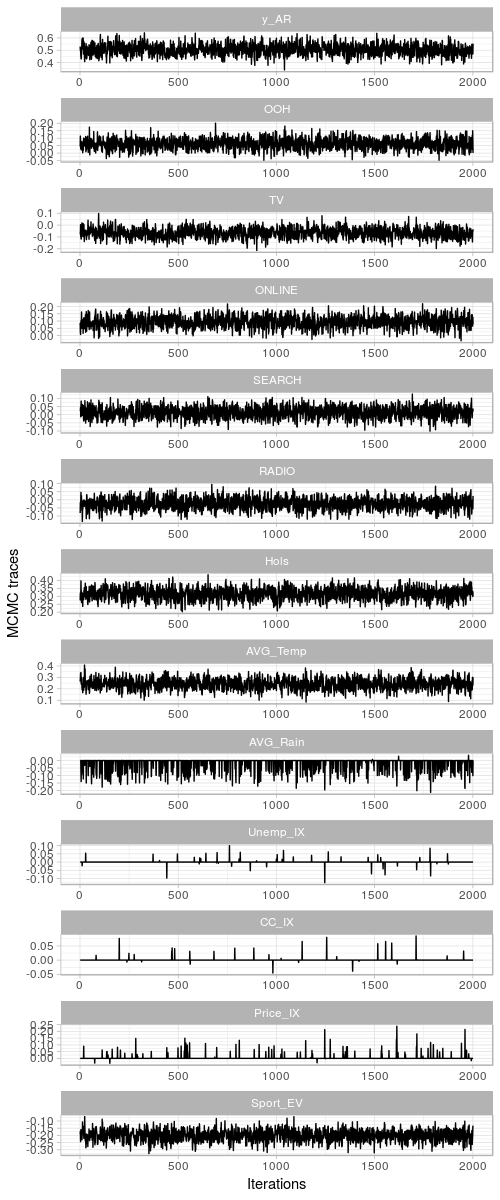
\includegraphics[scale=0.6]{figures/traces.png}
\caption{MCMC traces after a burn-in of 2000 iterations.}\label{fig:traces}
\end{figure}

